\newpage
\appendix

% chktex-file 21

\section{Appendix}

    \subsection{Nielsen's 10 usability heuristics}\label{appendix_nielsen}
    \begin{nielsenenumerate}
        \item Visibility of system status: the system should always keep users informed about what is going on, through appropriate feedback within reasonable time.
        \item Match between system and the real world: the system should speak the user's language, with words, phrases and concepts familiar to the user, rather than system-oriented terms. Follow real-world conventions, making information appear in a natural and logical order.
        \item User control and freedom: users often choose system functions by mistake and will need a clearly marked ``emergency exit'' to leave the unwanted state without having to go through an extended dialogue. Support undo and redo.
        \item Consistency and standards: users should not have to wonder whether different words, situations, or actions mean the same thing. Follow platform conventions.
        \item Error prevention: even better than good error messages is a careful design which prevents a problem from occurring in the first place. Either eliminate error-prone conditions or check for them and present users with a confirmation option before they commit to the action.
        \item Recognition rather than recall: minimize the user's memory load by making objects, actions, and options visible. The user should not have to remember information from one part of the dialogue to another. Instructions for use of the system should be visible or easily retrievable whenever appropriate.
        \item Flexibility and efficiency of use: accelerators unseen -- by the novice user -- may often speed up the interaction for the expert user such that the system can cater to both inexperienced and experienced users. Allow users to tailor frequent actions. % chktex 8
        \item Aesthetic and minimalist design: dialogues should not contain information which is irrelevant or rarely needed. Every extra unit of information in a dialogue competes with the relevant units of information and diminishes their relative visibility.
        \item Help users recognize, diagnose, and recover from errors: error messages should be expressed in plain language (no codes), precisely indicate the problem, and constructively suggest a solution.
        \item Help and documentation: even though it is better if the system can be used without documentation, it may be necessary to provide help and documentation. Any such information should be easy to search, focused on the user's task, list concrete steps to be carried out, and not be too large.
    \end{nielsenenumerate}

\newpage
\subsection{Patient JSON import specification}\label{json_import}

    The dashboard allows to import the medical data of multiple patients in a JSON format. The application only accepts the structure that is defined in this section. The root structure is an array in which each object contains the info of a patient:

\begin{lstlisting}[language=json,firstnumber=1]
[
    {
        // patient 1 info
    },
    {
        // patient 2 info
    },
    ...
    {
        // patient n info
    }
]
\end{lstlisting}

    Each patient object contains key-value pairs in which the key indicates the type of information it value contains. For example, the key ``info'' contains as a value an object containing the demographic information of the patient. The following example imports a patient with an allergy:
\begin{lstlisting}[language=json,firstnumber=1]
{
    "info": {
        "firstName": "Michael",
        "lastName": "Johnson",
        "nid": "123454321",
        "birth": "1983-02-09T11:23:00",
        "gender": "M",
        "bloodType": "O-",
        "height": "173",
        "address": "Largestreet 22, 12345 Bigtown",
        "phone": "0123/9890777",
        "smoker": "true"
    },
    "allergies": [
        {
            "name": "Nuts",
            "description": "Nausea",
            "severity": "2",
            "type": "Food",
            "date": "1998-12-04T00:00:00"
        }
    ]
}
\end{lstlisting}

    We now define each key and describe the structure of its value. By giving an example we define the structure. The comment after the key-value pair indicates the type of the value. The examples show all values within quotes. However, this does not mean they are all strings. All dates are entered as an ISO 8601 string value.

    \subsubsection{General patient information}

    The demographic information is imported by the controller of the patient information module (section~\ref{mod_patient_info}). The ``info'' key is the only key that is mandatory. The structure of the JSON object is as follows:

\begin{lstlisting}[language=json,firstnumber=1]
"info": {
    "firstName": "Michael", // String
    "lastName": "Johnson", // String
    "nid": "123454321", // String
    "birth": "1983-02-09T11:23:00", // String
    "gender": "M", // String, enum: ['M', 'F']
    "bloodType": "O-", // String, enum: ['O+', 'O-', 'A+', 'A-', 'B+', 'B-', 'AB+', 'AB-']
    "height": "173", // Integer
    "address": "Largestreet 22, 12345 Bigtown", // String
    "phone": "0123/9890777", // String
    "smoker": "true" // Boolean
}
\end{lstlisting}

    \subsubsection{Allergies}

    The allergy information is imported by the allergy module (section~\ref{mod_allergy}). The value of the key ``allergies'' is an array. Each object in this array defines an allergy. The object has the following structure:

\begin{lstlisting}[language=json,firstnumber=1]
{
    "name": "Nuts", // String
    "description": "Nausea", // String
    "severity": "2", // Integer
    "type": "Food", // String, enum: ['Food', 'Skin', 'Respiratory', 'Drug', 'Other']
    "date": "1998-12-04T00:00:00" // String
}
\end{lstlisting}

    \subsubsection{Vaccinations}

    The vaccination information is imported by the vaccination module (section
    \ref{mod_vaccination}). The value of the key ``vaccinations'' is an array. Each object in this array defines a vaccination. Each vaccination can have multiple entries, which are defined in the array of the key ``entries''. The object has the following structure:

\begin{lstlisting}[language=json,firstnumber=1]
{
    "name": "Hepatitis B", // String
    "description": "Liver disease.", // String
    "dateNext": "2019-03-23T16:30:00", // String
    "entries": [ // array of objects
        {
            "description": "1ste vaccination, patient was 13 months old.", // String
            "date": "2014-11-14T13:45:00" // String
        }
    ]
}
\end{lstlisting}



\newpage
\subsection{Usability test documents}\label{appendix_test_docs}

    \subsubsection{Informed consent: original (Dutch)}\label{appendix_test_consent}

    Note: the form was created in Microsoft Word and fit on exactly one page. The Hasselt University logo was located on the top right of the form.
    
    \vspace{6pt}
    \hrule
    \vspace{6pt}
    \noindent Beste vrijwilliger,\bigskip
    
    \noindent Dit formulier dient om u informatie te geven over de studie waar u aan gaat deelnemen. Op het einde vragen we u dit formulier te ondertekenen om uw vrijwillige deelname te bevestigen. U kan te allen tijde uw deelname aan de studie intrekken. Een ondertekend kopie van dit document wordt aan u meegegeven.\bigskip
    
    \noindent De data verkregen van u en de observatie wordt geanonimiseerd en niet verder verspreid buiten de grenzen van deze studie.\bigskip

    \noindent\textbf{Onderwerp: medisch dashboard met als focus per-pati\"{e}nt personalisatie}\bigskip

    \noindent Deze studie stelt een dashboard voor die een zorgverlener toelaat om per individuele pati\"{e}nt de nodige functionaliteit samen te stellen. Door ons prototype van het dashboard te testen, kunnen we de sterktes en zwaktes ervan identificeren. We testen het prototype en niet u, de gebruiker. U kunt dus niets verkeerd doen tijdens deze test.\bigskip

    \noindent Het verloop van deze test bestaat uit drie delen:
    \vspace{-\topsep}
    \begin{myenumerate}
        \item Vragenlijst betreffende persoonlijke gegevens en gebruikte medische software (5 \`{a} 10 min).
        \item Test van het prototype met behulp van een stappenplan (20 \`{a} 25 min).
        \item Interview en een vragenlijst om de gebruikerservaring te toetsen (10 min).
    \end{myenumerate}

    \noindent Voordat de test van het prototype van start gaat, krijgt u een korte uitleg omtrent het gebruik van het dashboard. Zodra de test begonnen is, wordt u geobserveerd. Indien er problemen of onduidelijkheden ontstaan mag u altijd vragen stellen. Tenslotte wordt u aangeraden om luidop te denken.\bigskip

    \noindent\textbf{Verklaring van toestemming}\bigskip

    \noindent Handtekening testpersoon:\quad\quad\quad\quad\quad\quad\quad Handtekening getuige:\bigskip\bigskip

    \noindent Naam: \rule{0.29\textwidth}{0.4pt} \quad\quad\quad\quad\quad Naam: \rule{0.29\textwidth}{0.4pt}\medskip

    \noindent Datum: \rule{0.15\textwidth}{0.4pt}\medskip

    \noindent\textbf{Contactgegevens:}\quad Naam:\hspace{10pt}Dennis Cardinaels\newline
    \hspace*{97pt}Email:\hspace{10pt}dennis.cardinaels@student.uhasselt.be\newline
    \hspace*{97pt}GSM\@:\hspace{13pt}0479 51 47 19

    \vspace{10pt}
    \hrule
    \vspace{6pt}

    \subsubsection{Pre-test questionnaire: original (Dutch)}\label{appendix_pretest}

    Description: In de eerste sectie worden enkele demografische gegevens van u verzameld. Daarna vragen we informatie omtrent het EPD (elektronische pati\"{e}ntendossier) dat momenteel in gebruik is.\bigskip

    \noindent\textbf{Persoonlijke informatie}\bigskip

    \noindent \(\bullet\) Geslacht*\footnote{A star indicates a mandatory question.}: \hspace{10pt} \(\circ\) Male\hspace{10pt}\(\circ\) Female\medskip

    \noindent \(\bullet\) Leeftijd*:\hspace{6pt}\rule{0.1\textwidth}{0.4pt}\medskip

    \noindent \(\bullet\) Wat is uw huidige jobtitel?*\hspace{6pt}\rule{0.4\textwidth}{0.4pt}\medskip

    \noindent \(\bullet\) Hoe lang werkt u al binnen de gezondheidszorgsector?*\hspace{6pt}\rule{0.2\textwidth}{0.4pt}\medskip

    \noindent \(\bullet\) Hoe ervaren bent u met computers?*
    \vspace{-6pt}
    \begin{center}
    Onervaren\hspace{20pt}\(\circ\)\hspace{20pt}\(\circ\)\hspace{20pt}\(\circ\)\hspace{20pt}\(\circ\)\hspace{20pt}\(\circ\)\hspace{20pt}Ervaren
    \end{center}

    \noindent \(\bullet\) Welke apparaten gebruikt u dagelijks?*
    \vspace{-8pt}
    \begin{multicols}{2}
        \begin{list}{\(\square\)}{} 
            \itemsep-0.3em 
            \item Computer/laptop
            \item Smartphone
            \item Tablet
            \item Andere: \rule{0.2\textwidth}{0.4pt}
        \end{list}
    \end{multicols}

    \noindent \(\bullet\) Welke apparaten gebruikt u enkele malen per week?*
    \vspace{-8pt}
    \begin{multicols}{2}
        \begin{list}{\(\square\)}{} 
            \itemsep-0.3em 
            \item Computer/laptop
            \item Smartphone
            \item Tablet
            \item Andere: \rule{0.2\textwidth}{0.4pt}
        \end{list}
    \end{multicols}

    \noindent \(\bullet\) Welke apparaten gebruikt u enkele malen per maand?*
    \vspace{-8pt}
    \begin{multicols}{2}
        \begin{list}{\(\square\)}{} 
            \itemsep-0.3em 
            \item Computer/laptop
            \item Smartphone
            \item Tablet
            \item Andere: \rule{0.2\textwidth}{0.4pt}
        \end{list}
    \end{multicols}

    \noindent\textbf{Elektronisch pati\"{e}ntendossier (EPD)}\bigskip

    \noindent \(\bullet\) Wat is de naam van het huidige EPD?*\hspace{6pt}\rule{0.4\textwidth}{0.4pt}\medskip

    \noindent \(\bullet\) Wordt het EPD op mobiele apparaten (smartphone/tablet) gebruikt?*
    \vspace{-6pt}
    \begin{center}
        \(\circ\) Ja\hspace{10pt}\(\circ\) Nee
    \end{center}

    \noindent \(\bullet\) Hoe lang is dit EPD in gebruik? (indien u dit niet weet, laat open)\hspace{6pt}\rule{0.1\textwidth}{0.4pt}\medskip

    \noindent \(\bullet\) Hoe tevreden bent u van het EPD?*
    \vspace{-6pt}
    \begin{center}
    Zeer ontevreden\hspace{20pt}\(\circ\)\hspace{20pt}\(\circ\)\hspace{20pt}\(\circ\)\hspace{20pt}\(\circ\)\hspace{20pt}\(\circ\)\hspace{20pt}Zeer tevreden
    \end{center}

    \noindent \(\bullet\) Het EPD is gebruiksvriendelijk.*
    \vspace{-6pt}
    \begin{center}
    Helemaal niet akkoord\hspace{10pt}\(\circ\)\hspace{20pt}\(\circ\)\hspace{20pt}\(\circ\)\hspace{20pt}\(\circ\)\hspace{20pt}\(\circ\)\hspace{10pt}Helemaal akkoord
    \end{center}

    \noindent \(\bullet\) Het EPD voldoet aan al mijn eisen.*
    \vspace{-6pt}
    \begin{center}
    Helemaal niet akkoord\hspace{10pt}\(\circ\)\hspace{20pt}\(\circ\)\hspace{20pt}\(\circ\)\hspace{20pt}\(\circ\)\hspace{20pt}\(\circ\)\hspace{10pt}Helemaal akkoord
    \end{center}

    \noindent \(\bullet\) Welke functies ontbreken in het EPD?\hspace{6pt}\rule{0.2\textwidth}{0.4pt}\medskip

    \noindent \(\bullet\) Het EPD kan aangepast worden naar eigen wens.*\hspace{10pt} \(\circ\) Ja\hspace{10pt}\(\circ\) Nee\medskip

    \noindent \(\bullet\) Indien `ja' op de vorige vraag, in welke mate? Is dit bijvoorbeeld per pati\"{e}nt\newline
    \hspace*{9pt}mogelijk?\hspace{6pt}\rule{0.3\textwidth}{0.4pt}\medskip

    \noindent \(\bullet\) Worden andere programma's in combinatie gebruikt met het EPD?*
    \vspace{-6pt}
    \begin{center}
        \(\circ\) Ja\hspace{10pt}\(\circ\) Nee
    \end{center}

    \noindent \(\bullet\) Indien `ja' op de vorige vraag, welke programma's?\hspace{6pt}\rule{0.2\textwidth}{0.4pt}

    \subsubsection{Post-test questionnaire: original (Dutch)}\label{appendix_posttest}

    Description: De volgende vragen toetsen uw ervaring met het prototype. Indien u nog extra opmerkingen hebt die niet in de enqu\^{e}te genoteerd kunnen worden, mag u dit altijd melden.\bigskip

    \noindent\textbf{Persoonlijke ervaring}\bigskip

    \noindent \(\bullet\) Algemene ervaring met het dashboard.*
    \vspace{-6pt}
    \begin{center}
    Zeer slecht\hspace{10pt}\(\circ\)\hspace{15pt}\(\circ\)\hspace{15pt}\(\circ\)\hspace{15pt}\(\circ\)\hspace{15pt}\(\circ\)\hspace{15pt}\(\circ\)\hspace{15pt}\(\circ\)\hspace{10pt}Zeer goed
    \end{center}

    \noindent \(\bullet\) Het dashboard is makkelijk om te gebruiken.*
    \vspace{-6pt}
    \begin{center}
    Helemaal niet akkoord\hspace{10pt}\(\circ\)\hspace{20pt}\(\circ\)\hspace{20pt}\(\circ\)\hspace{20pt}\(\circ\)\hspace{20pt}\(\circ\)\hspace{10pt}Helemaal akkoord
    \end{center}

    \noindent \(\bullet\) Het dashboard ziet er duidelijk uit.*
    \vspace{-6pt}
    \begin{center}
    Helemaal niet akkoord\hspace{10pt}\(\circ\)\hspace{20pt}\(\circ\)\hspace{20pt}\(\circ\)\hspace{20pt}\(\circ\)\hspace{20pt}\(\circ\)\hspace{10pt}Helemaal akkoord
    \end{center}

    \noindent \(\bullet\) De modules zien er duidelijk uit.*
    \vspace{-6pt}
    \begin{center}
    Helemaal niet akkoord\hspace{10pt}\(\circ\)\hspace{20pt}\(\circ\)\hspace{20pt}\(\circ\)\hspace{20pt}\(\circ\)\hspace{20pt}\(\circ\)\hspace{10pt}Helemaal akkoord
    \end{center}

    \noindent \(\bullet\) Alles is makkelijk terug te vinden in het dashboard.*\hspace{10pt} \(\circ\) Ja\hspace{10pt}\(\circ\) Nee\medskip

    \noindent \(\bullet\) Indien `nee' op de vorige vraag, wat was moeilijk om terug te vinden?\hspace{6pt}\rule{0.1\textwidth}{0.4pt}\medskip

    \noindent \(\bullet\) De modules dienden als een goed voorbeeld wat mogelijk is met het\newline
    \hspace*{9pt}dashboard.*
    \vspace{-6pt}
    \begin{center}
    Helemaal niet akkoord\hspace{10pt}\(\circ\)\hspace{20pt}\(\circ\)\hspace{20pt}\(\circ\)\hspace{20pt}\(\circ\)\hspace{20pt}\(\circ\)\hspace{10pt}Helemaal akkoord
    \end{center}

    \noindent \(\bullet\) Heeft u suggesties voor potenti\"{e}le modules?\hspace{6pt}\rule{0.3\textwidth}{0.4pt}\medskip

    \noindent \(\bullet\) Er zijn voldoende personalisatie mogelijkheden aanwezig in het dashboard.*
    \vspace{-6pt}
    \begin{center}
    Helemaal niet akkoord\hspace{10pt}\(\circ\)\hspace{20pt}\(\circ\)\hspace{20pt}\(\circ\)\hspace{20pt}\(\circ\)\hspace{20pt}\(\circ\)\hspace{10pt}Helemaal akkoord
    \end{center}

    \noindent \(\bullet\) Wat vond u goed/niet goed aan de personalisatie?\hspace{6pt}\rule{0.3\textwidth}{0.4pt}

    \subsubsection{Step-by-step plan: original (Dutch)}\label{appendix_test_steps}

    Note: the step-by-step plan was created in Google Docs and fit on exactly two pages.

    \vspace{6pt}
    \hrule
    \vspace{6pt}
    \noindent\textbf{Start}
    \vspace{-6pt}
    \begin{myenumerate}
        \item Log in als:
        \begin{myenumerate}
            \item Username: ``verpleger1''.
            \item Wachtwoord: ``dashboard''.
        \end{myenumerate}
        \item Selecteer pati\"{e}nt ``Kenny Martens''.
    \end{myenumerate}

    \noindent\textbf{Pati\"{e}nt Kenny Martens}\newline
    Achtergrond: Kenny is een account manager van een grote boekhouding firma. Zijn stressvolle job, sedentaire levensstijl en gewoonte om te roken hebben gezondheidsproblemen met zich meegebracht. Zo heeft hij regelmatig last van hartkloppingen en een hoge bloeddruk. Thuis moet Kenny regelmatig zijn gewicht, hartslag en bloeddruk meten met apparaten die de waardes doorsturen naar het elektronisch pati\"{e}ntendossier.\medskip

    \noindent Stappen:
    \vspace{-6pt}
    \begin{myenumerate}
        \item Bekijk het dashboard en open en sluit het zijpaneel.
        \item Pas een filter toe op de historiek van de pati\"{e}ntendata:
        \begin{myenumerate}
            \item Zet de startdatum op een week geleden en de einddatum op vandaag.
            \item Selecteer enkel de voorschrijvingen en de telemonitoring modules.
            \item Laat alle operaties geselecteerd staan.
        \end{myenumerate}
        \item Voeg een telemonitoring module toe dat de resterende breedte en hoogte van de pagina inneemt. Stel in:
        \begin{myenumerate}
            \item Toon bloeddrukwaarden en plot ze op de y-as.
            \item Selecteer data vanaf vandaag tot ongeveer een maand geleden.
            \item Bekijk de waarden van enkele datapunten op de lijngrafieken.
            \item Beschrijf de trend van de data op beide grafieken.
        \end{myenumerate}
        \item Open het zijpaneel en maak het pati\"{e}nteninformatie moduletje kleiner.
        \item Voeg een kleine telemonitoring module toe aan het zijpaneel:
        \begin{myenumerate}
            \item Selecteer de bloeddruk, hartslag en gewicht als parameters.
            \item Toon een samenvatting van de laatste 14 dagen.
        \end{myenumerate}
        \item Sleep de telemonitoring module zodat deze boven de huidige medicatie module staat.
        \vspace{10pt}
        \item Maak de webbrowser breder totdat het zijpaneel openklapt en ga naar de pati\"{e}ntenlijst.
        \item Selecteer pati\"{e}nt ``Jozefien Hendrix''.
    \end{myenumerate}

    \noindent\textbf{Pati\"{e}nt Jozefien Hendrix}\newline
    Achtergrond: Jozefien is een pas gepensioneerde dame die al heel haar leven zwaarlijvig is. Nu ze pas op pensioen is gegaan, is ze alarmerend aan het bij-komen. Om dit tegen te gaan, gaat ze regelmatig op controle bij de huisarts. Bij elke raadpleging past de huisarts haar medicatieschema aan en daarbovenop geeft hij suggesties voor waar ze op moet letten.\medskip

    \noindent Stappen:
    \vspace{-6pt}
    \begin{myenumerate}
        \item Bekijk de details van enkele voorschriften uit de lijst.
        \begin{myenumerate}
            \item Verwijder het voorschrift voor ``Furosemide''.
            \item Voeg een nieuw voorschrift toe:
            \begin{myenumerate}
                \item Selecteer medicijn ``Simvastatine'' en een dosering naar keuze.
                \item Zet de periode van het voorschrift van begin december tot eind december.
                \item Zijn er interacties? Zo ja, welke?
            \end{myenumerate}
        \end{myenumerate}
        \item Verwijder de allergie module en voeg in de plaats een workflow module toe.
        \begin{myenumerate}
            \item Laadt workflow ``Consultatieprocedure'' in.
            \item Verwijder de eerste stap ``Nieuwe pati\"{e}nt''.
            \item Voeg een nieuwe substap ``Medicatieschema controleren'' toe aan de ``Pre-consultatie'' stap.
        \end{myenumerate}
        \item Reset de checklijst.
        \begin{myenumerate}
            \item Voeg de taak ``Medicatie voorschrijven'' toe en vink deze aan.
            \item Voeg aan de taak ``Metingen uitvoeren'' een subtaak ``Gewicht'' toe.
        \end{myenumerate}
        \item In het zijpaneel, verberg de zuurstof parameter in de telemonitoring module.
        \vspace{10pt}
        \item Ga naar de pati\"{e}ntenlijst en selecteer pati\"{e}nt ``Bert Nieuwenhuize''.
    \end{myenumerate}

    \noindent\textbf{Pati\"{e}nt Bert Nieuwenhuize}\newline
    Achtergrond: Na een zwaar auto ongeluk, ligt Bert op de intensieve zorgafdeling. Bert heeft een hele waslijst aan allergie\"{e}n, medicatie dat hij inneemt en is niet helemaal up-to-date met zijn vaccinaties. Momenteel wordt hij behandeld door meerdere dokters en geobserveerd door verpleegkundigen. Het is dus belangrijk dat iedereen op de hoogte is van Bert zijn allergie\"{e}n, huidige medicatie, enzovoort. Echter zijn de gegevens in het EPD onvolledig, vergeleken met het papieren dossier dat het ziekenhuis in handen heeft.\medskip

    \noindent Stappen:
    \vspace{-6pt}
    \begin{myenumerate}
        \item Bij de allergie module, doe het volgende:
        \begin{myenumerate}
            \item Verander de reactiegraad van de ``koeienmelk'' allergie naar niveau 1.
            \item Voeg een ``Latex'' allergie (type ``Other'') toe met beschrijving ``Jeuk, last van luchtwegen, niezen'', reactiegraad 5 en de datum op vandaag.
        \end{myenumerate}
        \item Bekijk enkele inentingsdata van vaccinaties in de vaccinatiemodule.
        \begin{myenumerate}
            \item Verwijder de ``test'' vaccinatie.
            \item Voeg een nieuwe vaccinatie ``Hepatitis B''  met beschrijving ``Lever-ontsteking'' toe.
            \begin{myenumerate}
                \item Kies 12 januari als volgende inentingsdatum.
                \item Voeg een nieuwe historische vaccinatie toe met als beschrijving ``1ste vaccinatie, pati\"{e}nt was 12 jaar oud'' en de datum 11 april 1990.
            \end{myenumerate}
        \end{myenumerate}
        \item In de historiek van de pati\"{e}ntendata, pas de volgende filter toe:
        \begin{myenumerate}
            \item Zet de startdatum op 3 dagen geleden en de einddatum op vandaag.
            \item Selecteer de allergie en vaccinatie module.
            \item Selecteer alle operaties buiten ``import''.
            \item Bekijk enkele details van de historiek.
        \end{myenumerate}
    \end{myenumerate}

    \newpage
    \subsubsection{Screenshots taken at the start of each scenario}\label{appendix_test_screens}

    \begin{figure}[h!]
        \centering
        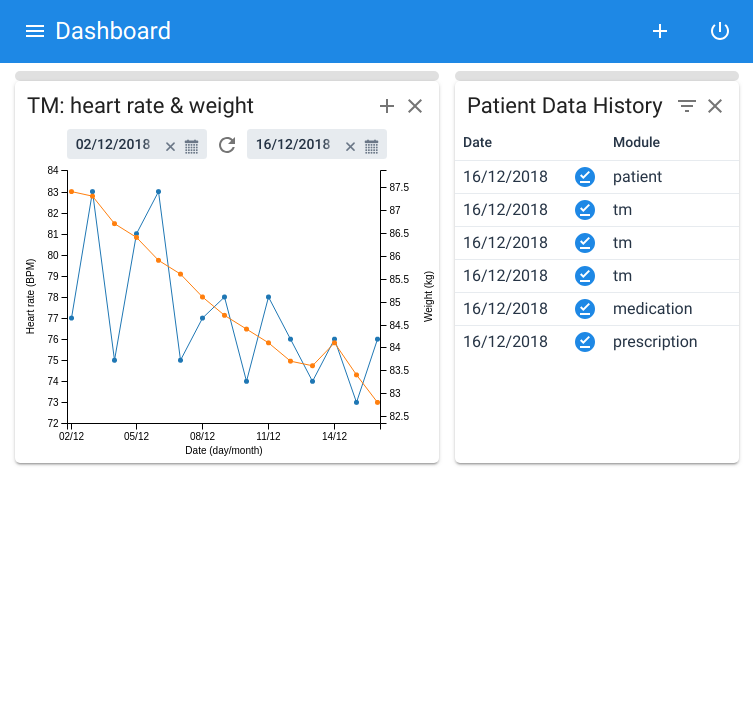
\includegraphics[width=0.65\textwidth]{chapters/appendix/test_kenny}
        \caption{The dashboard of Kenny at the start of his scenario. There is still space left for other modules below.}
    \end{figure}
    \begin{figure}[h!]
        \centering
        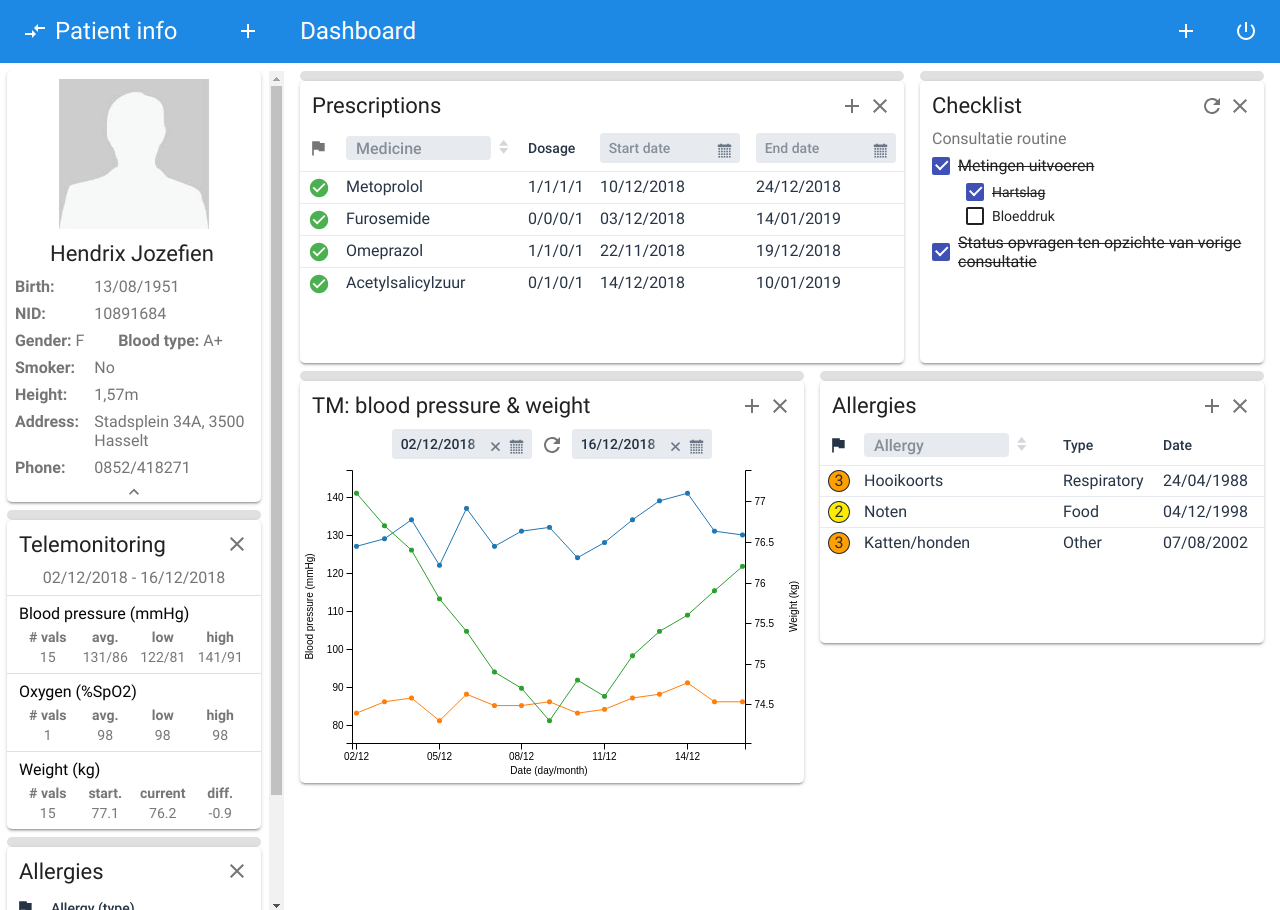
\includegraphics[width=0.85\textwidth]{chapters/appendix/test_jozefien}
        \caption{The dashboard of Jozefien at the start of her scenario.}
    \end{figure}
    \begin{figure}[h!]
        \centering
        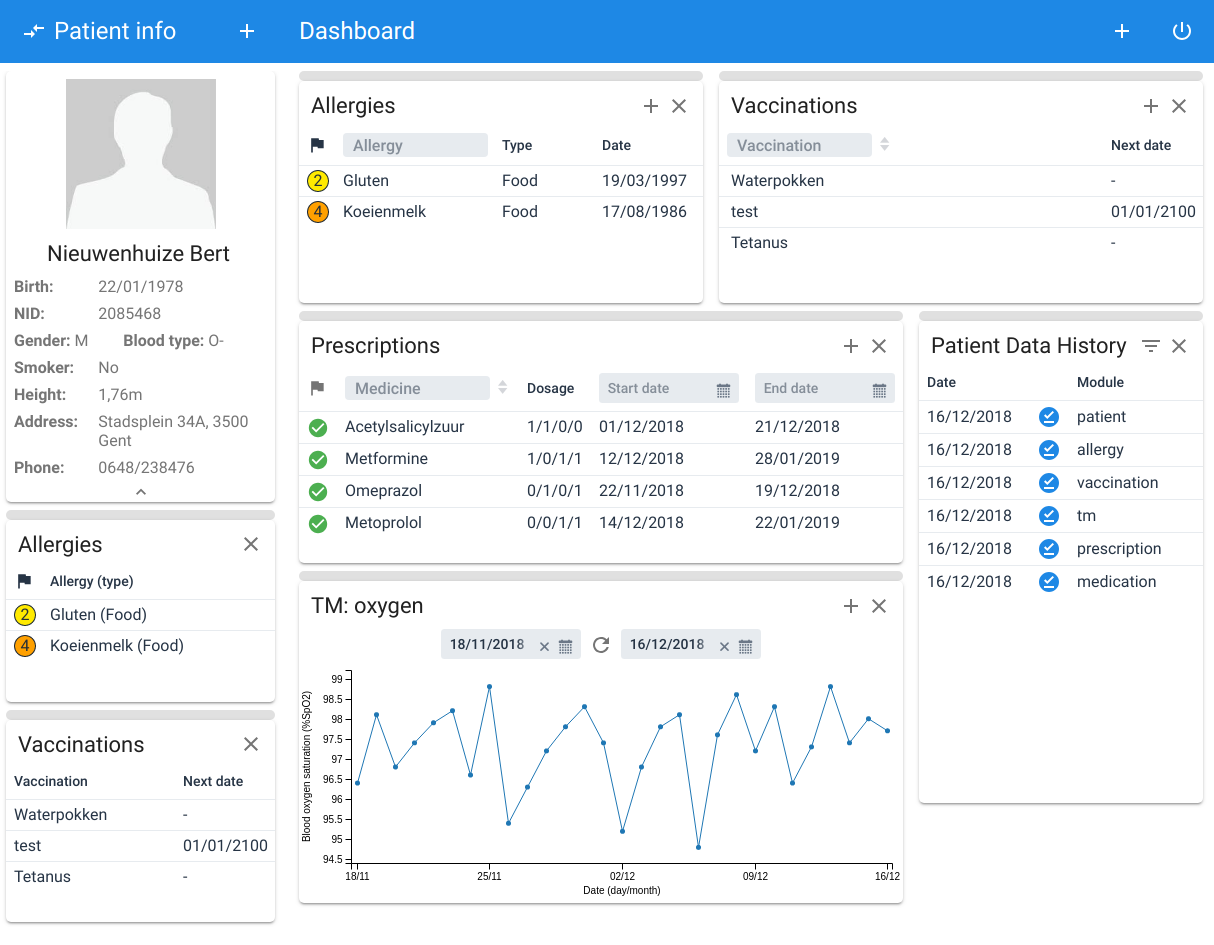
\includegraphics[width=1\textwidth]{chapters/appendix/test_bert}
        \caption{The dashboard of Bert at the start of his scenario.}
    \end{figure}